% ============================================================
% DOE Genesis Mission CFP 2026 — Pre-Proposal
% SVF: Structured Validation Framework for Trustworthy AI in Scientific Software
% Focus Area: 18E — Trustworthy AI for Scientific Software
% ============================================================

\documentclass{files/proposalnsf}

\usepackage[utf8]{inputenc}
\usepackage[T1]{fontenc}
\usepackage{graphicx}
\usepackage{hyperref}
\usepackage{microtype}
\usepackage{cite}
\usepackage{enumitem}
\usepackage{tikz}
\usetikzlibrary{arrows.meta,positioning}
\setlist{nosep, leftmargin=1.5em, topsep=0.2em}

\usepackage{xspace}
\usepackage{xcolor}

\newcommand{\todo}[1]{{\color{red}\bfseries [[TODO: #1]]}}

\newcommand{\tool}{\textcolor{blue}{\texttt{cool\_tool}}\xspace}

\newcommand{\approach}{\textcolor{blue}{\textit{approach}}\xspace}

\newcommand{\proposalEleven}{\textbf{Provenance-Aware Agentic Knowledge Graphs}}
\newcommand{\proposalEighteen}{\textbf{Provenance-Aware Agentic Knowledge Graphs}}
\newcommand{\proposalNineteen}{\textbf{Provenance-Aware Agentic Knowledge Graphs}}


\newcommand{\ie}{\textit{i.e.,}\xspace}

\newcommand{\eg}{\textit{e.g.,}\xspace}

\newcommand{\etal}{\textit{et al.}\xspace}

\begin{document}

\begin{center}
    \large{\proposalEighteen} \\ \vspace{0.5pt}
\footnotesize{PI: Chris Brown, Computer Science, Virginia Tech} \\
\footnotesize{Co-PI: Xuan Wang, Computer Science, Virginia Tech} \\
\footnotesize{Co-PI: Scott T. Steinmetz, Sandia National Labs} \\
\footnotesize{GRA: Jason Cusati, Computer Science, Virginia Tech}
\end{center}

\small{\noindent\textbf{Focus Area:} 18 -- HPC Code Curation, Translation, and Development for Accelerated Scientific Discoveries} \hfill \\
\small{\textbf{Topic:} E. Trustworthy AI for Scientific Software}

\subsubsection*{Project Summary / Abstract}

Trustworthy AI for scientific software demands systematic guarantees of \textit{numerical correctness, reproducibility, provenance tracking, interpretable diagnostics, and uncertainty quantification}---the five properties explicitly enumerated in DOE 18E. Yet existing evaluation frameworks for AI-assisted software development assess these properties only in isolation. Retrieval-augmented generation (RAG) benchmarks~\cite{Lewis2020RAG} measure retrieval accuracy but not claim provenance. Frameworks such as RAGAS~\cite{Es2023RAGAS}, ARES~\cite{SaadFalcon2023ARES}, and TruLens~\cite{TruEra2023TruLens} evaluate individual RAG pipeline components but do not address compound agentic systems---those where multiple agents coordinate over heterogeneous knowledge, invoke external tools, and produce cumulative outputs such as scientific code artifacts. As AI-assisted HPC code development matures, this evaluation gap becomes a reliability gap: there is no principled way to certify that an AI-generated scientific code is grounded in correct evidence, reproducibly derived, or accompanied by meaningful uncertainty estimates~\cite{Ji2023HallucinationSurvey}.

\begin{figure}[t]
    \centering
    \resizebox{\columnwidth}{!}{%
    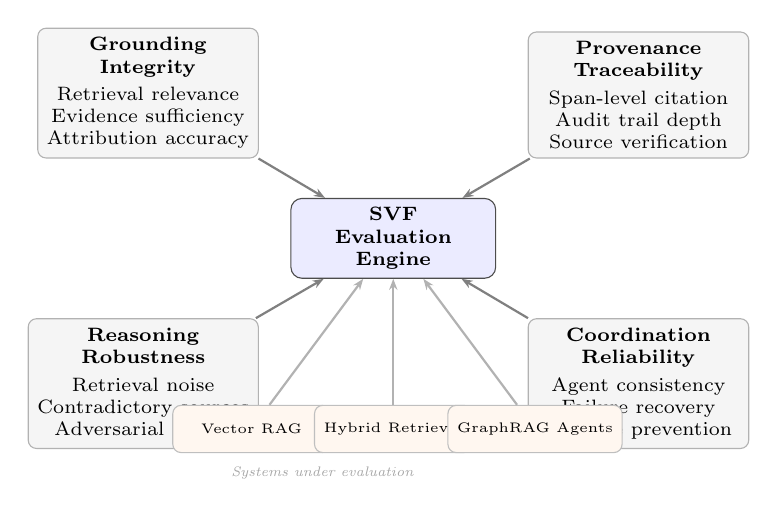
\begin{tikzpicture}[
        node distance=0.4cm and 0.3cm,
        dimbox/.style={rectangle, rounded corners=3pt, draw=gray!60, fill=gray!8, minimum width=2.8cm, minimum height=1.6cm, align=center, font=\scriptsize},
        centerbox/.style={rectangle, rounded corners=4pt, draw=black!70, fill=blue!8, minimum width=2.6cm, minimum height=0.9cm, align=center, font=\scriptsize\bfseries},
        sysbox/.style={rectangle, rounded corners=3pt, draw=gray!50, fill=orange!6, minimum width=2.0cm, minimum height=0.6cm, align=center, font=\tiny},
        arr/.style={-{Stealth[length=4pt]}, thick, gray!60},
        dimarr/.style={-{Stealth[length=4pt]}, thick, black!50},
    ]
        % Center
        \node[centerbox] (svf) {SVF\\Evaluation\\Engine};

        % Four dimensions
        \node[dimbox, above left=0.5cm and 0.4cm of svf] (gi) {\textbf{Grounding}\\\textbf{Integrity}\\[2pt]Retrieval relevance\\Evidence sufficiency\\Attribution accuracy};
        \node[dimbox, above right=0.5cm and 0.4cm of svf] (pt) {\textbf{Provenance}\\\textbf{Traceability}\\[2pt]Span-level citation\\Audit trail depth\\Source verification};
        \node[dimbox, below left=0.5cm and 0.4cm of svf] (rr) {\textbf{Reasoning}\\\textbf{Robustness}\\[2pt]Retrieval noise\\Contradictory sources\\Adversarial inputs};
        \node[dimbox, below right=0.5cm and 0.4cm of svf] (cr) {\textbf{Coordination}\\\textbf{Reliability}\\[2pt]Agent consistency\\Failure recovery\\Cascade prevention};

        % Systems under test (bottom)
        \node[sysbox, below=1.6cm of svf, xshift=-1.8cm] (rag) {Vector RAG};
        \node[sysbox, below=1.6cm of svf] (hybrid) {Hybrid Retrieval};
        \node[sysbox, below=1.6cm of svf, xshift=1.8cm] (graph) {GraphRAG Agents};

        % Arrows from dimensions to SVF
        \draw[dimarr] (gi) -- (svf);
        \draw[dimarr] (pt) -- (svf);
        \draw[dimarr] (rr) -- (svf);
        \draw[dimarr] (cr) -- (svf);

        % Arrows from systems to SVF
        \draw[arr] (rag) -- (svf);
        \draw[arr] (hybrid) -- (svf);
        \draw[arr] (graph) -- (svf);

        % Labels
        \node[font=\tiny\itshape, gray!70, below=0.05cm of rag, xshift=0.9cm] {Systems under evaluation};
    \end{tikzpicture}
    }%
    \caption{\textbf{SVF Evaluation Framework.} The Structured Validation Framework evaluates knowledge-grounded agentic systems across four dimensions directly aligned with DOE 18E requirements. Systems under test are assessed via OpenTelemetry GenAI-instrumented execution traces~\cite{OpenTelemetryGenAI2024}.}
    \label{fig:framework}
    \vspace{-0.5em}
\end{figure}

This project proposes the \textbf{Structured Validation Framework (SVF)}, systematic evaluation infrastructure for knowledge-grounded and multi-agent AI systems operating on scientific software tasks. SVF evaluates along four complementary dimensions that directly operationalize 18E requirements (Figure~\ref{fig:framework}): (1)~\textbf{grounding integrity}---whether retrieved evidence is relevant, sufficient, and correctly attributed to generated claims (correctness proxy); (2)~\textbf{provenance traceability}---whether reasoning chains can be audited from output back to specific source spans (reproducibility and audit trail); (3)~\textbf{reasoning robustness}---whether systems degrade gracefully under retrieval noise, contradictory sources, and adversarial perturbations (diagnostic signal for failure modes); and (4)~\textbf{coordination reliability}---whether multi-agent systems maintain consistency under component failures and cascade error propagation (uncertainty quantification for system-level behavior). Unlike post-hoc benchmarks, SVF embeds validation as a first-class component of agent execution pipelines using OpenTelemetry GenAI semantic conventions~\cite{OpenTelemetryGenAI2024}, producing structured trace signals consumable by existing observability infrastructure.

Our prior work motivates SVF directly. Brown \& Cusati~\cite{brown2025esem} demonstrate that generative AI tools propagate evidence inconsistently in software engineering contexts; Cusati \& Brown~\cite{cusati2026fose} show that research knowledge accumulates without structured tracking mechanisms. SVF builds the measurement infrastructure needed to make AI-assisted scientific software development systematically trustworthy---and to identify precisely \textit{where} and \textit{why} it fails.

Expected outcomes include: the SVF evaluation toolkit with OpenTelemetry instrumentation; a benchmark suite for scientific software tasks targeting all four dimensions; empirical comparison of vector RAG, hybrid retrieval, and graph-augmented agent systems~\cite{Edge2024GraphRAG}; and deployment guidelines for embedding SVF in production AI-assisted HPC code development workflows.

\subsubsection*{Research Plan}

\paragraph{Introduction.}
HPC scientific software development is central to DOE's scientific mission. The 18E challenge identifies the core problem: existing AI coding tools lack trustworthiness---they cannot provide numerical correctness guarantees, reproducibility of outputs, provenance of generated code back to authoritative knowledge, interpretable diagnostics when they fail, or principled uncertainty estimates. This is not merely an accuracy problem. A scientific code generated by an AI agent may produce plausible-looking results while silently violating physical conservation laws, introducing non-reproducible nondeterminism, or deriving logic from a hallucinated source~\cite{Ji2023HallucinationSurvey}. Without systematic evaluation infrastructure, practitioners cannot distinguish trustworthy AI assistance from fluent-but-wrong output.

Existing evaluation frameworks do not close this gap. RAGAS~\cite{Es2023RAGAS} and ARES~\cite{SaadFalcon2023ARES} evaluate retrieval quality and answer faithfulness for single-turn RAG pipelines. TruLens~\cite{TruEra2023TruLens} extends this to simple agent chains. None address compound multi-agent systems where agents coordinate over heterogeneous scientific knowledge, invoke domain simulation tools, and produce cumulative artifacts spanning code, data, and documentation. Self-RAG~\cite{Asai2024SelfRAG} introduces retrieval self-reflection but does not measure coordination failure or uncertainty propagation. SVF is designed to fill this gap: it provides the evaluation substrate that makes trustworthy AI-assisted scientific software development measurable, comparable, and improvable.

\paragraph{Objectives.}
\begin{enumerate}
    \item Design and implement the SVF evaluation toolkit with formal operational specifications for all four dimensions.
    \item Develop OpenTelemetry GenAI instrumentation for capturing structured execution traces from agent workflows.
    \item Construct a benchmark suite of scientific software tasks targeting grounding integrity, provenance traceability, reasoning robustness, and coordination reliability.
    \item Validate SVF against RAGAS, ARES, and TruLens to characterize the evaluation gap for compound agentic systems.
    \item Demonstrate that SVF signals predict real-world trustworthiness failures in AI-generated scientific software.
\end{enumerate}

\paragraph{Research Questions.}
\begin{itemize}
    \item \textbf{RQ1:} What evaluation dimensions are necessary and sufficient to assess trustworthiness of compound agentic AI systems producing scientific software artifacts?
    \item \textbf{RQ2:} How do existing frameworks (RAGAS, ARES, TruLens) fail to capture reliability properties that SVF measures, and at what rate do these gaps produce false positive trustworthiness assessments?
    \item \textbf{RQ3:} How do SVF metrics correlate with detected errors in AI-generated scientific code when validated against domain expert review and automated testing?
    \item \textbf{RQ4:} How can validation loops be embedded within agent orchestration to detect and recover from grounding failures in real time?
\end{itemize}

\paragraph{Detailed Research Plan.}

\textit{Phase 1 (Months 1--3): Framework Design and Instrumentation.}
We will formally specify each SVF dimension with quantitative metrics: grounding integrity as retrieval precision/recall against human-annotated relevance judgments; provenance traceability as audit trail depth (fraction of output tokens traceable to specific source spans); reasoning robustness as accuracy degradation under adversarial retrieval perturbations; and coordination reliability as cascade failure rate and mean time to recovery under fault injection. We will implement an OpenTelemetry GenAI instrumentation layer that intercepts agent execution at tool-call and LLM-inference boundaries, emitting structured spans aligned with emerging GenAI semantic conventions~\cite{OpenTelemetryGenAI2024}. We will survey the existing evaluation landscape (RAGAS, ARES, TruLens, and related frameworks) and systematically characterize which 18E properties each covers and which it leaves unmeasured, building the theoretical foundation for SVF's gap-filling contribution.

\textit{Phase 2 (Months 4--6): Benchmark Construction and Baseline Comparison.}
We will construct a fault injection benchmark for multi-agent scientific software systems, implementing three fault types: (1)~\textit{tool drop}---silently discard tool responses to measure recovery behavior; (2)~\textit{retrieval corruption}---inject incorrect or contradictory documents into retrieved context; and (3)~\textit{response delay}---introduce latency to surface timeout and cascade failure modes. We will construct an adversarial retrieval test set specifically targeting reasoning robustness in scientific code generation contexts, where adversarial documents contain physically plausible but incorrect numerical values. We will then run baseline comparison: apply RAGAS, ARES, and TruLens to the same benchmark tasks and compare coverage, false positive rate, and actionable diagnostic signal against SVF. We predict SVF will detect trustworthiness failures invisible to component-level metrics, particularly in the provenance traceability and coordination reliability dimensions.

\textit{Phase 3 (Months 7--9): Evaluation, Generalization, and Deployment Guidelines.}
We will apply SVF to evaluate three AI system architectures on scientific software tasks: vector-only RAG, hybrid dense+sparse retrieval, and graph-augmented agentic systems~\cite{Edge2024GraphRAG}. For each system, we will correlate SVF dimension scores with ground-truth error rates identified through expert review and automated test suites. Longitudinal evaluation will test whether SVF predicts downstream code correctness and reproducibility across software evolution cycles. We will develop deployment guidelines for embedding SVF in production AI-assisted HPC code development pipelines, including minimal instrumentation overhead targets and threshold calibration procedures. All SVF toolkit components, benchmarks, and results will be released as open-source artifacts.

\paragraph{Team Roles.}
\textbf{PI Chris Brown} leads framework design, evaluation methodology, and SE-domain benchmark task construction. \textbf{Co-PI Xuan Wang} leads ML systems instrumentation, multi-agent coordination evaluation design, and adversarial robustness benchmarking. \textbf{Co-PI Scott T. Steinmetz} (Sandia National Labs) provides HPC scientific software domain expertise and validates SVF signals against DOE-relevant code correctness benchmarks. \textbf{GRA Jason Cusati} implements the SVF toolkit, constructs benchmark suites, and executes experimental evaluation and baseline comparisons.

\bibliographystyle{IEEEtran}
\bibliography{references}

\end{document}
